\documentclass[border=10pt]{standalone}

\usepackage{tikz}
\usepackage{tikzsymbols}
\usetikzlibrary{calc,patterns,shapes.geometric}

\def\centerarc[#1](#2)(#3:#4:#5){\draw[#1] ($(#2)+({#5*cos(#3)},{#5*sin(#3)})$) arc (#3:#4:#5);}

\begin{document}
	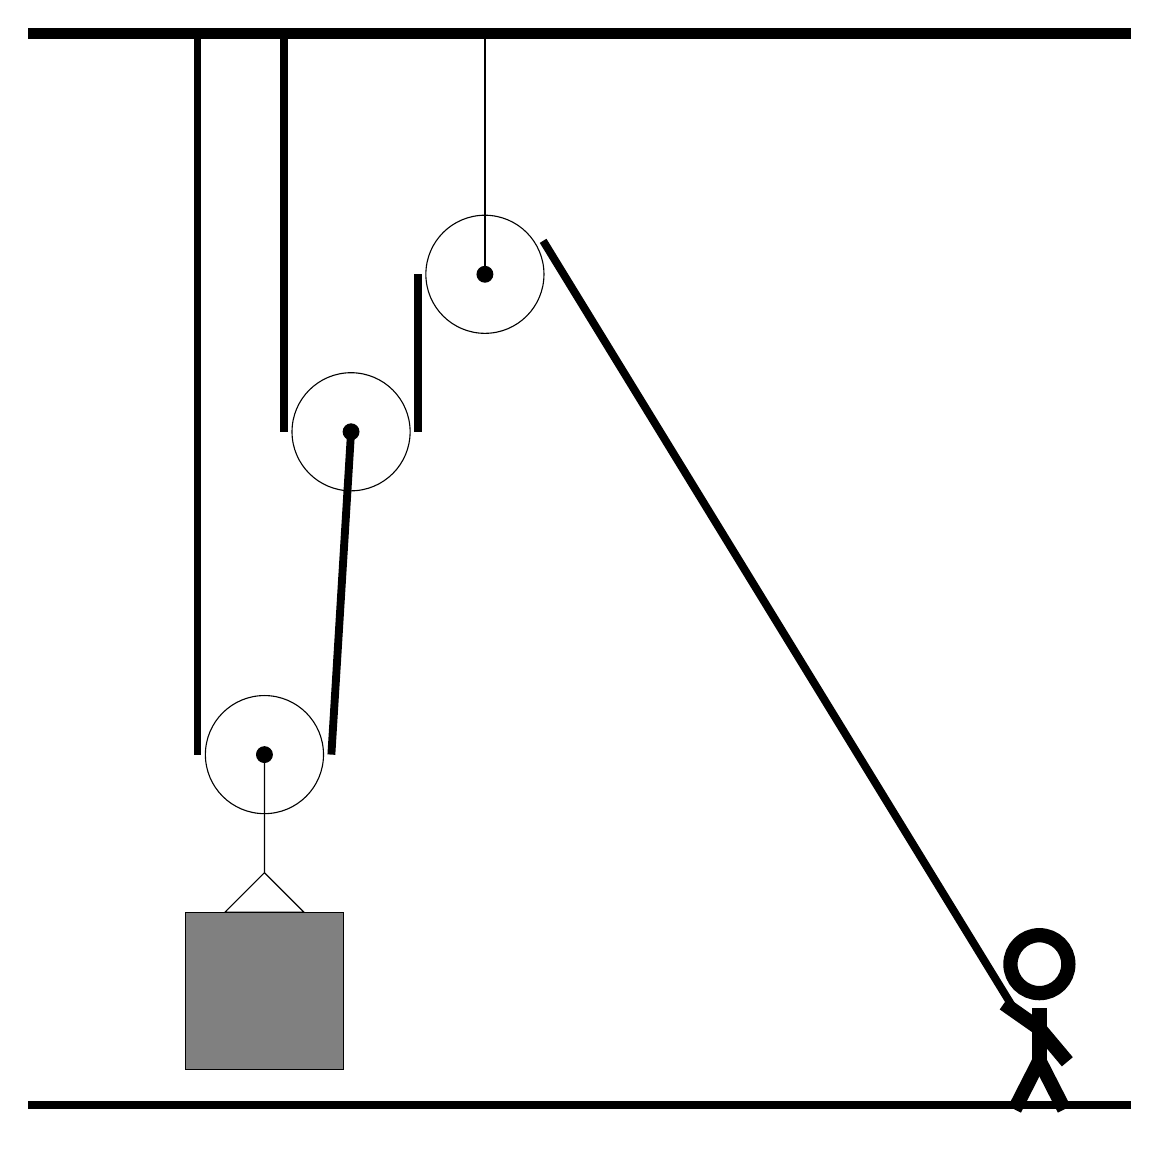
\begin{tikzpicture}
		%%%%% START %%%%%
		\draw[fill=black] (-2, 10) rectangle (12, 10.125);
		
		\draw (1, 0.9) circle (0.75);
		\draw[fill=black] (1, 0.9) circle (0.1);
		
		\draw (2.1, 5.0) circle (0.75);
		\draw[fill=black] (2.1, 5.0) circle (0.1);
		
		\draw (3.8, 7.0) circle (0.75);
		\draw[fill=black] (3.8, 7.0) circle (0.1);
		\draw[thick] (3.8, 7.0) -- (3.8, 10);
		
		\draw (1, 0.9) -- (1, -0.6) -- (0.5, -1.1) -- (1.5, -1.1) -- (1, -0.6);
		\draw[fill=black!50] (0, -1.1) rectangle (2, -3.1);
		
		\draw[line width=1mm] (0.15, 10) -- (0.15, 0.9);
		\centerarc[line width=1mm](1, 0.9)(180:360:0.85);
		\draw[line width=1mm](1.85, 0.9) -- (2.1, 5.0);
		\draw[line width=1mm] (1.25, 10) -- (1.25, 5.0);
		\centerarc[line width=1mm](2.1, 5.0)(180:360:0.85);
		\draw[line width=1mm](2.95, 5.0) -- (2.95, 7.0);
		\centerarc[line width=1mm](3.8, 7.0)(30:180:0.85);
		\draw[line width=1mm] (4.539, 7.425) -- (10.5, -2.3);
		
		\node at (10.8, -2.5) {\Strichmaxerl[10][-35][-50]};
		
		\draw[fill=black] (-2, -3.5) rectangle (12, -3.6);
		%%%%% END %%%%%
	\end{tikzpicture}
\end{document}